%!TEX root = main.tex

\chapter{Applications of LTE Atmospheres}

\section{Continuum Opacity}

\subsection{Sun}

At the point at which $\tau(5000\:{\Angstrom}) = 2/3$ in the
solar atmosphere we have $n_\mathrm{H} \approx 1.1 \times
10^{17}$, $n_e \approx 4 \times 10^{13}\:\mathrm{cm^{-3}}$
and $T \approx 6200$. We can use the Saha equation to
determine the fraction of ionized hydrogen as
\begin{align}
\frac{n_\mathrm{H^+}}{n_\mathrm{H^0}}
\approx 
2.6 \times 10^{-4},
\end{align}
in which we have used $U_\mathrm{H^0} \approx 2$ and
$U_\mathrm{H^+} = 1$. The hydrogen in the solar atmosphere
is overwhelmingly neutral. 

\begin{figure}
\centering
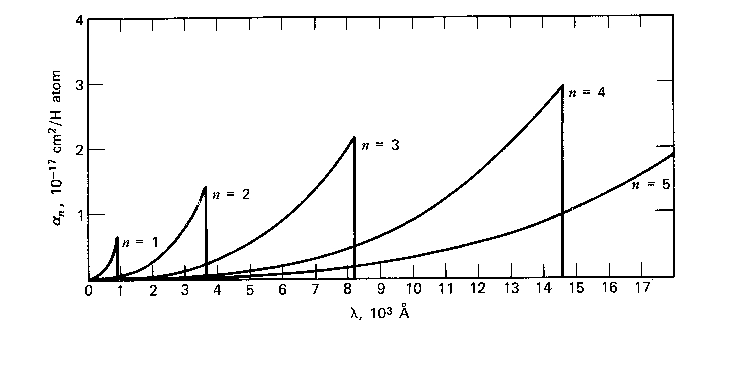
\includegraphics[width=0.7\linewidth]{figures/h-zero.pdf}
\caption{The opacity of $\mathrm{H}^0$. The ordinate is the cross-section per neutral hydrogen atom in the given excited state.}
\end{figure}

The continuum opacity of neutral hydrogen depends on the
degree of excitation. For example, the Lyman continuum at
$\lambda < 912\:{\Angstrom}$ corresponds to ionizations from
the $n=1$ level, the Balmer continuum for $\lambda <
3647\:{\Angstrom}$ corresponds to ionizations from the $n=2$
level, and the Paschen continuum for $\lambda <
8206\:{\Angstrom}$ corresponds to ionizations from the $n=3$
level. In the optical, we are concerned with the Paschen
continuum, and so we need to calculate the excitation of the
$n=3$ level
\begin{align}
\frac{n_{\mathrm{H}^0_{n=3}}}{n_{\mathrm{H^0}}}
\approx
1.4 \times 10^{-9}.
\end{align}
Thus, although almost all of the hydrogen in the Solar
atmosphere is neutral, almost none of it is in a state in
which it can contribute to the opacity in the visual.

We can also calculate the relative abundance of
$\mathrm{H^-}$. This is a stable bound state consisting of a
proton and two electrons and has an ionization potential of
0.754 eV. It has no bound excited states above the ground
state and so we have $U_\mathrm{H^-} = 1$, because the
electrons in the ground state must have opposite spins. We
find
\begin{align}
\frac{n_\mathrm{H^-}}{n_\mathrm{H^0}}
\approx 
3.5 \times 10^{-8}.
\end{align}
Thus, $\mathrm{H^-}$ is very rare in the solar atmosphere,
but is roughly 25 times more common than neutral hydrogen in
the $n=3$ state. Since the continuum cross-sections for
bound-free transitions are roughly similar ($2.4 \times
10^{-17}\:\mathrm{cm^{2}}$ for neutral hydrogen at the
Paschen edge and about $4 \times 10^{-17}\:\mathrm{cm^{2}}$
for $\mathrm{H^-}$ at its peak at roughly 8500 {\Angstrom}),
bound-free absorption by $\mathrm{H^-}$ dominates the
optical continuum opacity.

\begin{figure}
\centering
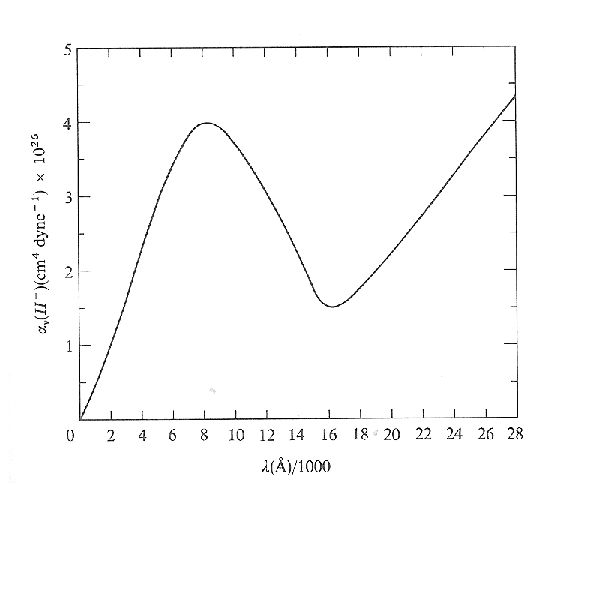
\includegraphics[width=0.7\linewidth]{figures/h-minus.pdf}
\caption{The opacity of $\mathrm{H}^-$ at $6300\;\mathrm{K}$. The ordinate is the cross-section per neutral hydrogen atom and per unit electron pressure $n_e kT$. The opacity below $1.6\;\micron$ is dominated by bound-bound absorption and above $1.6\;\micron$ by bound-free absorption.}
\end{figure}

\begin{figure}
\centering
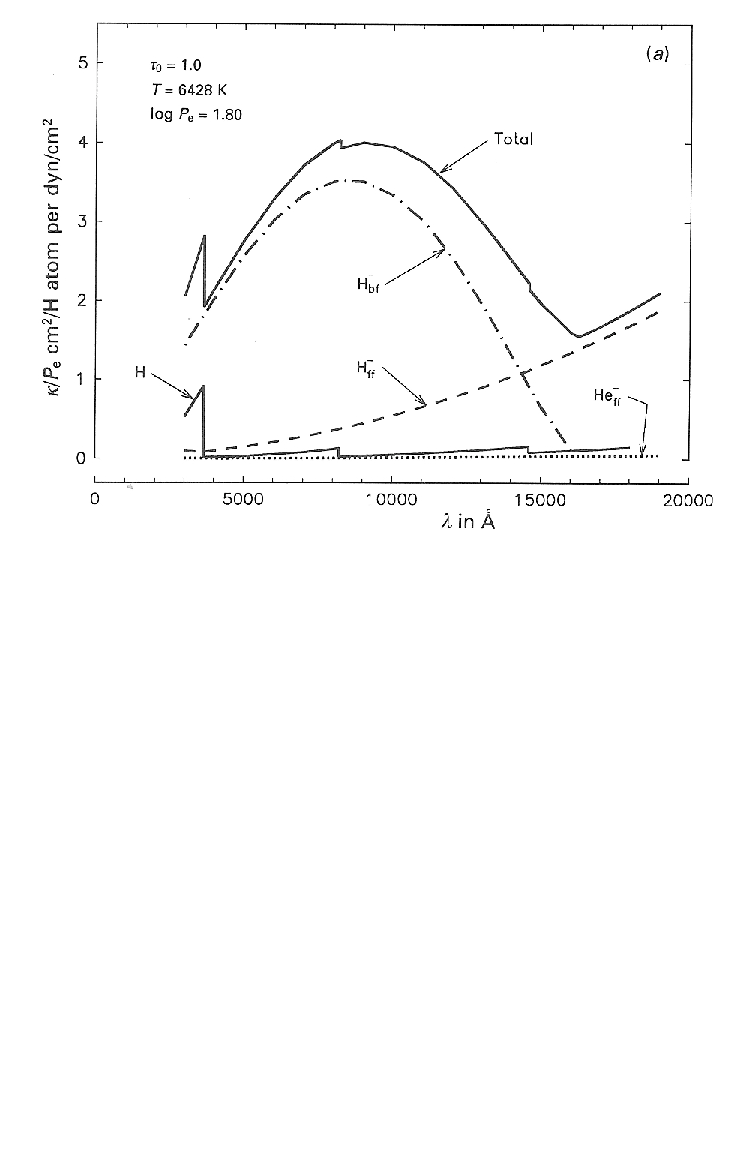
\includegraphics[width=0.7\linewidth]{figures/opacity-a.pdf}
\caption{The opacity in the optical under conditions typical of the solar photosphere. The opacity is dominated by $\mathrm{H}^-$.}
\end{figure}

Since the absorption coefficient is the product of the
cross-section per absorber and the density of absorbers, we
might expect that it should be linear in the total density.
However, consideration of $\mathrm{H^-}$ absorption in cool
stars shows that this is not always the case. We can write
the Saha equation for $\mathrm{H^-}$ as
%\comment{This is normally
%expressed as the mass-opacity depending linearly on the
%electron pressure.}
\begin{align}
\alpha 
&= 
a_\mathrm{H^-} n_\mathrm{H^-}\\
&= 
a_\mathrm{H^-}\frac{n_\mathrm{H^0} n_e}{n_\mathrm{S}}e^{\chi/kT}\\
&\propto n n_e.
\end{align}
In the Sun, $n_p
\approx 2.9 \times 10^{13}\:\mathrm{cm^{-3}} \approx 0.75 n_e$.
Thus, in the Sun and hotter stars the dominant source of
electrons is hydrogen. The Saha
equation for ionization of hydrogen then gives $n_e n_p
\propto n$ and since $n_e \approx n_p$ this leads to $n_e \propto
n^{1/2}$. The absorption coefficient then becomes
\begin{align}
\alpha \propto n^{3/2}.
\end{align}
This is more complicated than the simple $\alpha \propto
n$ that we would expect of the relative fraction of
absorbers was constant. This behaviour leads to important
differences between the atmospheres of cool giants (low
density) and dwarfs (higher density).
%\comment{This is normally
%expressed as the mass-opacity depending linearly on the
%electron pressure.}
We'll see a slightly different
dependence of the $\mathrm{H^-}$ opacity on density in
cooler stars below.

Above 1.65 {\micron}, $\mathrm{H^-}$ continues to dominate,
but now by free-free absorption. In the ultraviolet above
912 {\Angstrom}, ionization of Mg, Al, Si, and C and
Rayleigh scattering dominate the continuum opacity. Line
blanketing is important in the blue and the ultraviolet. Below
912 {\Angstrom} absorption by neutral hydrogen from the
$n=1$ ground state dominates.
%\comment{Figure for opacity. We
%need to discuss the form of the H$^0$ and H$^-$ opacity somewhere.}

\begin{figure}
\centering
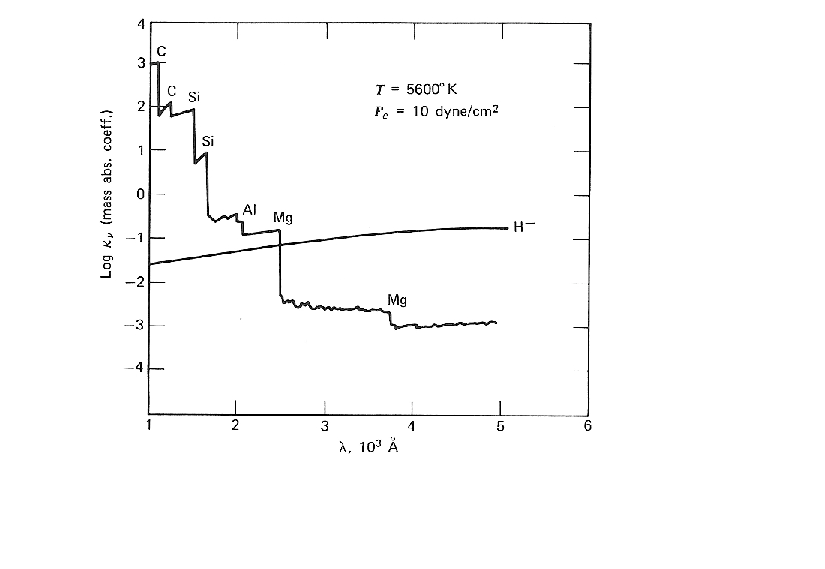
\includegraphics[width=0.7\linewidth]{figures/opacity-uv.pdf}
\caption{The opacity in the UV and optical under conditions typical of the solar photosphere. The UV opacity is dominated by bound-free absorption of Mg, Al, Si, and C.}
\end{figure}

\newslide

\subsection{Hotter Stars}

% Kurucz 1979 8000/4.5 model at tau_500 = 0.64
% T = 8800 n_e = 7.5e14 n_n = 2.0e16 n_H = 1.8e16

% n_S = 3.989e21

\begin{figure}
\centering
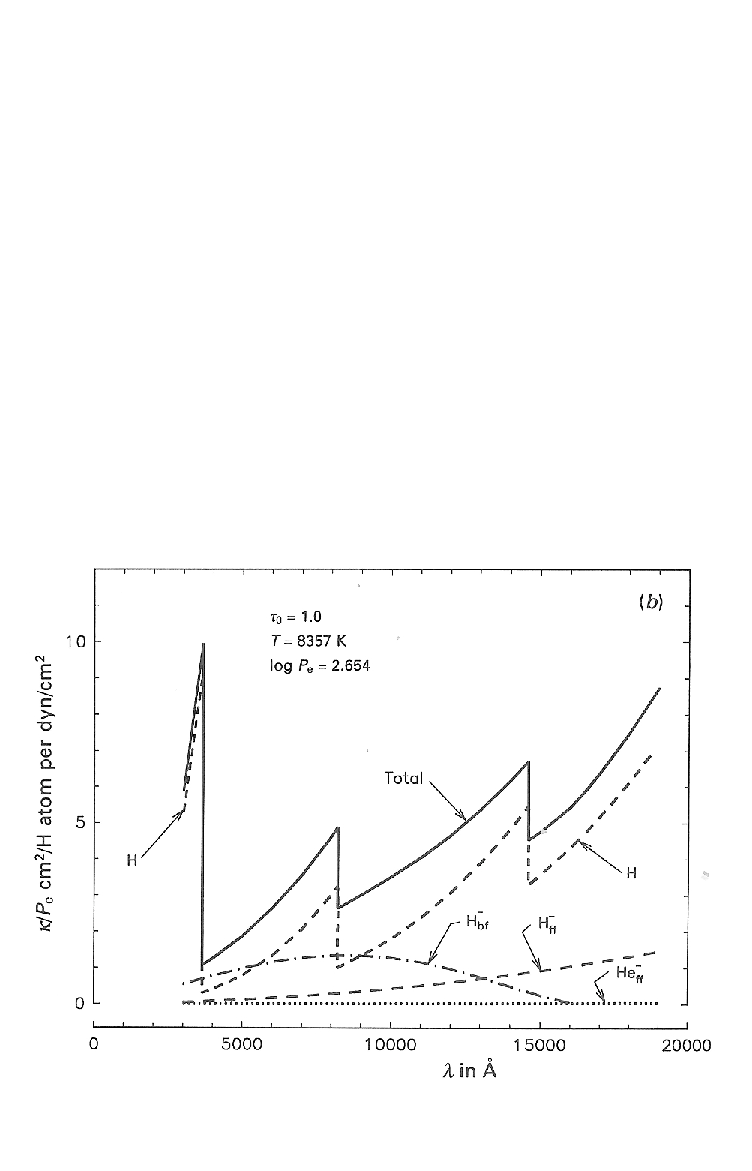
\includegraphics[width=0.7\linewidth]{figures/opacity-b.pdf}
\caption{The opacity in the optical under conditions typical of a late A dwarf. The opacity is dominated by $\mathrm{H}^-$ immediately above the Balmer jump and $\mathrm{H}^0$ immediately below the Balmer jump.}
\end{figure}

\begin{figure}
\centering
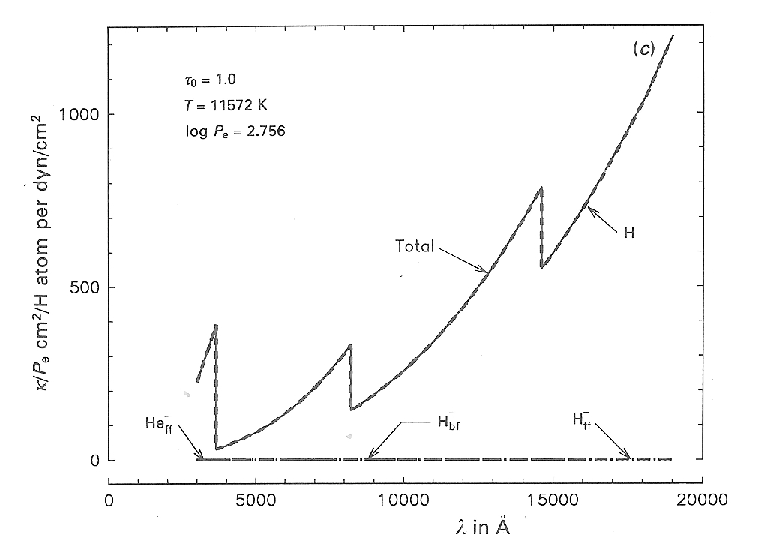
\includegraphics[width=0.7\linewidth]{figures/opacity-c.pdf}
\caption{The opacity in the optical under conditions typical of a late B dwarf. The opacity is dominated by $\mathrm{H}^0$ both immediately above and immediately below the Balmer jump.}
\end{figure}

A stars are hotter then the Sun, so the same point at which
$\tau(5000\:{\Angstrom}) = 2/3$ in the atmosphere of an A
dwarf with $\Teff \approx 8000\:\mathrm{K}$ would have
$n_\mathrm{H} \approx 1.8
\times 10^{16}$, $n_e \approx 7.5 \times
10^{14}\:\mathrm{cm^{-3}}$ and $T \approx 8800\:\mathrm{K}$.
Under these conditions, hydrogen is still largely neutral
with
\begin{align}
\frac{n_\mathrm{H^+}}{n_\mathrm{H^0}}
\approx
4.4 \times 10^{-2}.
\end{align}
However, the degree of ionization is now quite significant
-- almost 5\% compared to less than 0.03\% in the Sun -- and
so hydrogen supplies almost all of the electrons and we have
$n_\mathrm{H^+} \approx n_e$.

The abundance of $\mathrm{H^-}$ is also higher than in the
Sun with
\begin{align}
\frac{n_\mathrm{H^-}}{n_\mathrm{H^0}} \approx 2.5 \times 10^{-7}.
\end{align}
However, the abundance of neutral hydrogen in the $n=3$
level is also higher, with
\begin{align}
\frac{n_{\mathrm{H}^0_{n=3}}}{n_\mathrm{H^0}} \approx 1.1 \times 10^{-6}.
\end{align}
In these stars, absorption by the Paschen continuum is more
important than bound-free absorption by $\mathrm{H^-}$. This
trend increases through the A stars, but eventually hydrogen
becomes sufficiently ionized that first $\mathrm{He}{0}$
becomes important in the B stars and finally
$\mathrm{He}{+}$ becomes important in the O
stars. Electron scattering is also
important in O stars.

%\comment{Check this.}

At points at which the bound-free opacity is small, such as
just redward of the Balmer jump in early A and late B stars,
electron scattering opacity can be important. In the
ultraviolet, metals such as C, N, O, Ne, and Si continue to
be important.

%\comment{Check this.}

\newslide

\subsection{Cooler Stars}

$\mathrm{H^-}$ continues to be an important source of
opacity in stars cooler than the Sun. In these stars, the
ionization fraction of hydrogen is very low, and the
principal source of electrons is ionization of metals, and
so $n_e \propto x_\mathrm{M} n$, where $x_\mathrm{M}$ is the
fractional metal abundance. We then have
\begin{align}
\alpha \propto x_\mathrm{M} n^2.
\end{align}
Again, this is more complicated than the simple $\alpha
\propto n$ that we would expect of the relative fraction of
absorbers was constant. This behaviour leads to important
differences between the atmospheres of cool metal-poor and
metal-rich stars.

In stars cooler than mid-M, molecular hydrogen and its ions
can exist. H$_2$ itself does not absorb in the
optical, but H$_2^+$ and H$_2^-$
can be important. Much more important, though, is line
blanketing by first metallic lines and then by molecules.

%\comment{H$_2$ absorbs in the UV?}

\newslide

\section{Balmer Jump}

\begin{figure}
\footnotesize
\begin{tikzpicture}
\begin{axis}[
   xlabel={$ \lambda$ [nm]},
   ylabel={$\log F_\lambda$ $[\mathrm{W\,m^{-3}}]$},
   ymin=15.2,
   ymax=18.8,
   minor y tick num=4,
   xmin=300,
   xmax=600,
   minor x tick num=4, 
]
\addplot[black] table[x index=0,y index=1]{kurucz/Flambda-fp00t6000g50k0odfnew.dat};
\addplot[black] table[x index=0,y index=1]{kurucz/Flambda-fp00t7000g50k0odfnew.dat};
\addplot[black] table[x index=0,y index=1]{kurucz/Flambda-fp00t8500g50k0odfnew.dat};
\addplot[black,thick] table[x index=0,y index=1]{kurucz/Flambda-fp00t10000g50k0odfnew.dat};
\addplot[black] table[x index=0,y index=1]{kurucz/Flambda-fp00t12000g50k0odfnew.dat};
\addplot[black] table[x index=0,y index=1]{kurucz/Flambda-fp00t15000g50k0odfnew.dat};
\addplot[black] table[x index=0,y index=1]{kurucz/Flambda-fp00t20000g50k0odfnew.dat};
\end{axis}
\end{tikzpicture}
\caption{Emergent fluxes for ATLAS9 model atmospheres for $\log g = 5.0$ and $\Teff = 6000$, 7000, 8500, 10000 (thick), 12000, 15000, and 20000 K. Note that slope of the Paschen continuum (above 370 nm) becomes bluer with increasing temperature whereas the strength of the Balmer jump at 365 nm first increases and then decreases with effective temperature.}
\label{figure-atlas-teff}
\end{figure}

\begin{figure}
\footnotesize
\begin{tikzpicture}
\begin{axis}[
   xlabel={$ \lambda$ [nm]},
   ylabel={$\log F_\lambda$ $[\mathrm{W\,m^{-3}}]$},
   ymin=15.2,
   ymax=17.8,
   minor y tick num=3,
   xmin=300,
   xmax=600,
   minor x tick num=4, 
]
\addplot[black,thick] table[x index=0,y index=1]{kurucz/Flambda-fp00t7500g50k0odfnew.dat};
%\addplot[black] table[x index=0,y index=1]{kurucz/Flambda-fp00t7500g40k0odfnew.dat};
\addplot[black] table[x index=0,y index=1]{kurucz/Flambda-fp00t7500g30k0odfnew.dat};
%\addplot[black] table[x index=0,y index=1]{kurucz/Flambda-fp00t7500g20k0odfnew.dat};
\addplot[black] table[x index=0,y index=1]{kurucz/Flambda-fp00t7500g10k0odfnew.dat};
\end{axis}
\end{tikzpicture}
\caption{Emergent fluxes for ATLAS9 model atmospheres for $\log g = 1.0$, 3.0, and 5.0 (thick) and $\Teff = 7500$ K. Note that for stars of this temperature, the strength of the Balmer jump at 365 nm increases as the surface gravity decreases.}
\label{figure-atlas-logg-fg}
\end{figure}

\begin{figure}
\footnotesize
\begin{tikzpicture}
\begin{axis}[
   xlabel={$ \lambda$ [nm]},
   ylabel={$\log F_\lambda$ $[\mathrm{W\,m^{-3}}]$},
   ymin=16.2,
   ymax=18.8,
   minor y tick num=3,
   xmin=300,
   xmax=600,
   minor x tick num=4, 
]
\addplot[black,thick] table[x index=0,y index=1]{kurucz/Flambda-fp00t14000g50k0odfnew.dat};
%\addplot[black] table[x index=0,y index=1]{kurucz/Flambda-fp00t7500g40k0odfnew.dat};
\addplot[black] table[x index=0,y index=1]{kurucz/Flambda-fp00t14000g40k0odfnew.dat};
%\addplot[black] table[x index=0,y index=1]{kurucz/Flambda-fp00t7500g20k0odfnew.dat};
\addplot[black] table[x index=0,y index=1]{kurucz/Flambda-fp00t14000g30k0odfnew.dat};
\end{axis}
\end{tikzpicture}
\caption{Emergent fluxes for ATLAS9 model atmospheres for $\log g = 3.0$, 4.0, and 5.0 (thick) and $\Teff = 14000$ K. Note that for stars of this temperature, the strength of the Balmer jump at 365 nm does not depend strongly on the surface gravity.}
\label{figure-atlas-logg-ba}
\end{figure}


The Balmer jump at 3647 {\Angstrom} is an interesting
diagnostic of conditions in the stellar atmosphere. It
depends largely on the ratio of the opacities on either side
of 3647 {\Angstrom}. If the opacities are similar, the
continuum on both sides of the jump will be formed at
similar places in the atmosphere and so will be smooth and
not display a large jump. If the opacity on the blue side is
larger, the continuum here will be formed higher in the
atmosphere at cooler temperatures than the continuum on the
red side, and we would expect a large jump.

In F and G stars ($\Teff \approx 5000$--7500~K), the opacity longward of the jump is
largely due to H$^-$ whereas the opacity shortward of the
jump is due to both H$^-$ and bound-free absorption from the
$n=2$ level of H$^0$. The ratio of opacities is then
\begin{align}
\frac{\alpha(3647^-\:{\Angstrom})}{\alpha(3647^+\:{\Angstrom})}
&\approx
\frac{a_\mathrm{H^-} n_\mathrm{H^-} + a_{\mathrm{H}^0_{n=2}}
n_{\mathrm{H}^0_{n=2}}}
{a_\mathrm{H^-} n_\mathrm{H^-}}\\
&= 1 +
\frac{a_{\mathrm{H}^0_{n=2}}}{a_\mathrm{H^-}}
\frac{n_{\mathrm{H}^0_{n=2}}}{n_\mathrm{H^-}}
\end{align}
If we use the Saha and Boltzmann equations to determine the
relative densities of H$^-$ and H$^0$ in the $n=2$ state, we
can write
\begin{align}
\frac{\alpha(3647^-\:{\Angstrom})}{\alpha(3647^+\:{\Angstrom})}
&\approx
1 +
\left(\frac{a_{\mathrm{H}^0_{n=2}}}{a_\mathrm{H^-}}\right)
\left(\frac{8n_\mathrm{S}(T)e^{-(\chi_\mathrm{H^-} + E_{n=2})/kT}}{n_e}\right)
.
\end{align}
We can see then that the Balmer jump depends on both the
temperature and the electron density and can be used to
determine one given the other. The jump becomes stronger
with increasing temperature (recall that $n_\mathrm{S}
\propto T^{3/2}$) and with lower density. We would expect
it to strengthen towards earlier spectral classes and
towards decreasing surface gravity. This is exactly what is
observed in Figures~\ref{figure-atlas-teff}, \ref{figure-atlas-logg-fg}, and \ref{figure-balmer-jump}
 for effective temperatures of 5000--7500~K appropriate for FG stars.

\begin{figure}
\centering
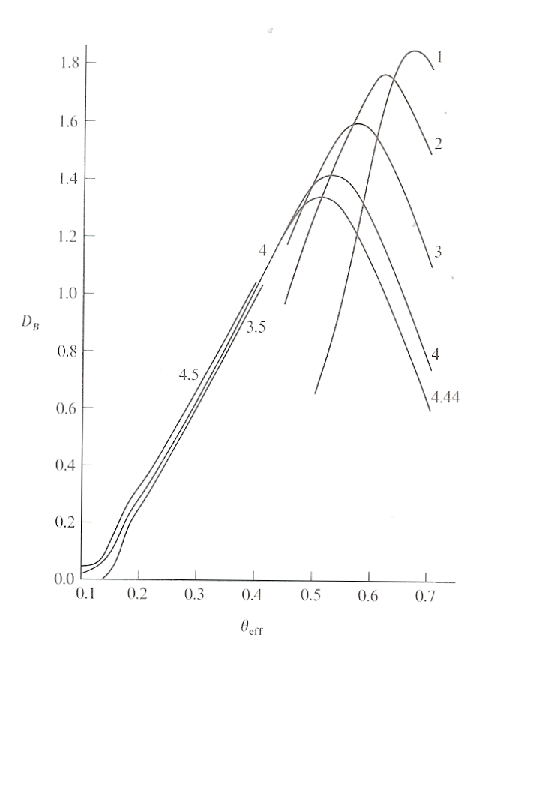
\includegraphics[width=0.8\linewidth]{figures/balmer-jump.pdf}
\caption{The Balmer jump $D_B \equiv 2.5 \log [F_\lambda(3647+)/F_\lambda(3647-)]$ calculated from LTE model atmospheres as a function of inverse effective temperature $\theta_\mathrm{eff} \equiv (5040\;\mathrm{K})/T_\mathrm{eff}$. The curves are labelled with $\log g$. Note that the Balmer jump depends on temperature and gravity for stars cooler than about $10,000\;\mathrm{K}$ but only on temperature for hotter stars.}
\label{figure-balmer-jump}
\end{figure}

For dwarf stars hotter than about 9000 K, the excitation of
the $n=3$ level is sufficiently large that that Paschen
continuum overtakes H$^-$ bound-free absorption as the
principal source of opacity longward of the Balmer jump. In
these stars,
\begin{align}
\frac{\alpha(3647^-\:{\Angstrom})}{\alpha(3647^+\:{\Angstrom})}
&\approx
\frac
{a_{\mathrm{H}^0_{n=3}} n_{\mathrm{H}^0_{n=3}} + a_{\mathrm{H}^0_{n=2}} n_{\mathrm{H}^0_{n=2}}}
{a_{\mathrm{H}^0_{n=3}} n_{\mathrm{H}^0_{n=3}}}\\
&\approx
1 + \left(
\frac
{a_{\mathrm{H}^0_{n=2}}}{a_{\mathrm{H}^0_{n=3}}}
\right)
\left(\frac{4}{9}e^{1.89\mathrm{eV}/kT}\right),
\end{align}
where the factor of $4/9$ comes from the relative
degeneracies (8 and 18) of the $n=2$ and $n=3$ levels and
1.89 eV is the energy difference between the $n=2$ and $n=3$
levels. Here the Balmer jump depends on temperature and not
density, and furthermore is a decreasing function of
temperature. This is seen in Figures~\ref{figure-atlas-teff}, \ref{figure-atlas-logg-ba}, and \ref{figure-balmer-jump} for effective temperatures of 9000--25,000~K appropriate for BA stars.

At higher temperatures and at the low densities encountered
in supergiants, electron scattering becomes important, first
on the red side of the jump and then even on the blue side.
In these stars, the Balmer jump again becomes a function of
both density and temperature.

\newslide

\section{Strömgren Photometry}

\begin{table}
\centering
\caption{Strömgren Filters}
\label{table:stromgren-filters}
\medskip
\begin{tabular}{cccc}
\hline
Filter	&Name&$\bar\lambda$ (nm)&$\Delta\lambda$ (nm)\\
\hline
$u$     &ultraviolet	&350&30\\
$v$     &violet		&411&19\\
$b$     &blue			&467&18\\
$y$     &yellow		&547&23\\
\hline
\end{tabular}
\end{table}

Strömgren defined a four-color $uvby$ photometric system based on intermediate width filters ($\Delta\lambda$ of $18$--30~nm compared to $160$--210~nm for the Johnson $UBV$ filters). As we can see in Figure~\ref{figure-uvby-balmer-jump}, the $u$ filter lies in the Balmer continuum below the Balmer jump and the $vby$ filters lie in the Paschen continuum above the Balmer jump. The $y$ magnitude of a star is closely correlated to the $V$ magnitude. The Strömgren filters were designed specifically to determine the parameters of stars. Their advantage compared to the Johnson filters is that they are much better attuned the the spectral features of stars; for example, the Strömgren $u$ filter is completely below the Balmer jump, whereas the Johnson $U$ filter straddles the Balmer jump.

Photometry with Strömgren filters is normally presented in terms of the $y$ magnitude, the $b-y$ color, and the $c_1$ and $m_1$ indices, which are defined by
\begin{align}
c_1 \equiv (u-v) - (v-b)
\intertext{and}
m_1 \equiv (v - b) - (b - y).
\end{align}
Note that $c_1$ and $m_1$ are differences between adjacent colors. Since colors measure in some sense the slope (first derivative) of a spectrum, the difference between two colors measures the curvature (second derivative) of a spectrum.

The $b-y$ color measures slope in Paschen continuum, which as we have see is well-correlated with the effective temperature for BAFG stars (e.g., in Figure~\ref{figure-atlas-teff}). Thus, $b-y$ is an effective temperature indicator in these stars.

The $c_1$ index measures the curvature in the $uvb$ region; the Balmer jump falls between $u$ and $v$, so $c_1$ will measure the strength of the Balmer jump (see also Figure~\ref{figure-uvby-balmer-jump}). Thus, $c_1$ is a surface gravity indicator for FG stars and an effective temperature indicator in BA stars.

Figure~\ref{figure-uvby-calibration} shows a calibration of $b-y$ and $c_1$ for effective temperature and gravity. It shows that for temperatures from 5500 to 8000~K, we can determine both the effective temperature and the surface gravity. Above 8000~K, we lose the ability to discriminate surface gravity from $c_1$. (We will shortly see how we can extend the Strömgren system to remedy this deficiency.)

The $m_1$ index measures the curvature in the $vby$ region. This region lies in the Paschen continuum, so at first it might appear that there should be little variation in the curvature. However,  in F and G stars, $v$ lies in a region that has several iron lines as well as the CN bands at $4142\,\Angstrom$ and $4215\,\Angstrom$, whereas $b$ and $y$ lie in regions that are largely free of lines (see also Figure~\ref{figure-uvby-metallicity}). Thus, differences in curvature in this region can be caused by variations in metallicity, as increasing metallicity reduced the flux in the $v$ filter more than in the $b$ and $y$ filters. Thus, $m_1$ is a metallicity indicator in F and G stars.

\begin{table}
\caption{Strömgren Diagnostics in BAFG Stars}
\begin{center}
\begin{tabular}{lcc}
\hline
Measurement&BA&FG\\
\hline
$b-y$&$\Teff$&$\Teff$\\
$c_1 = (u-v)-(v-b)$&$\Teff$&$\log g$\\
$m_1 = (v-b)-(b-y)$&&$Z$\\
\hline
\end{tabular}
\end{center}
\end{table}

\begin{figure}
\footnotesize
\begin{tikzpicture}
\begin{axis}[
   xlabel={$\lambda\:[\mathrm{nm}]$},
   ylabel={Normalized $S$},
   ymin=0,
   ymax=1,
   minor y tick num=3,
   xmin=300,
   xmax=600,
   minor x tick num=4,
]
\addplot[black] table{figures/stroemgren-u.dat};
\addplot[black] table{figures/stroemgren-v.dat};
\addplot[black] table{figures/stroemgren-b.dat};
\addplot[black] table{figures/stroemgren-y.dat};
\addplot[black,thick] table[x index=0,y index=1]{kurucz/Flambda-fp00t10000g50k0odfnew-norm.dat};
\end{axis}
\end{tikzpicture}
\caption{The Strömgren $uvby$ filters compared to the flux from a model atmosphere with $\Teff = 10,000$ K and $\log g = 5.0$. Notice that the $u$ filter is below the Balmer jump at 346~nm wherease the $vby$ filters are above it, which allows $c_1 \equiv (u-v)-(v-b)$ to be used as a indicator of the strength of the Balmer jump.}
\label{figure-uvby-balmer-jump}
\end{figure}

\begin{figure}
\centering
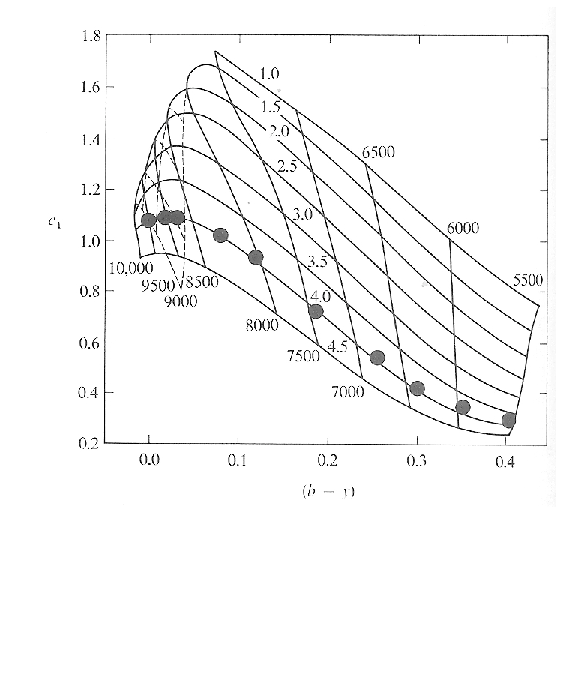
\includegraphics[width=0.5\linewidth]{figures/stromgren.pdf}
\caption{The $c_1$ index as a function of $b-y$. The grid shows the projection of a grid of LTE model atmospheres with different effective temperatures and gravities. The dots show the observed values of stars on the main sequence (which have $\log g\approx 4$). For stars between $8000\;\mathrm{K}$ (A5) and $5500\;\mathrm{K}$ (G7), the colors depend unambiguously on the effective temperature and gravity. Above $8000\;\mathrm{K}$, the relation between colors and effective temperature and surface gravity is double valued.}
\label{figure-uvby-calibration}
\end{figure}

\begin{figure}
\footnotesize
\begin{tikzpicture}
\begin{axis}[
   xlabel={$\lambda\:[\mathrm{nm}]$},
   ylabel={Normalized $S$},
   ymin=0,
   ymax=1,
   minor y tick num=3,
   xmin=300,
   xmax=600,
   minor x tick num=4,
]
\addplot[black] table{figures/stroemgren-u.dat};
\addplot[black] table{figures/stroemgren-v.dat};
\addplot[black] table{figures/stroemgren-b.dat};
\addplot[black] table{figures/stroemgren-y.dat};
%\addplot[black,thick] table[x index=0,y index=1]{kurucz/Flambda-fp00t10000g50k0odfnew-norm.dat};
%\addplot[black,thick] table[x index=0,y index=1]{kurucz/Flambda-fp00t7500g50k0odfnew-norm.dat};
\addplot[black,thick] table[x index=0,y index=1]{kurucz/Flambda-fp00t6000g50k0odfnew-norm.dat};
\end{axis}
\end{tikzpicture}
\caption{The Strömgren $uvby$ filters compared to the flux from a model atmosphere with $\Teff = 6000$ K and $\log g = 5.0$. Notice the strong metal absorption lines in the $v$ filter around 410 nm, which allows $m_1 \equiv (v-b)-(b-v)$ to be used as a metallicity indicator for FG stars.}
\label{figure-uvby-metallicity}
\end{figure}

%\section{Notes and Further Reading}

